
\section*{Kapitel 1 - Das einfache lineare Regressionsmodell}

\begin{multicols*}{3}

\tikzstyle{mybox} = [draw=black, fill=white, very thick,
    rectangle, rounded corners, inner sep=10pt, inner ysep=10pt]
\tikzstyle{fancytitle} =[fill=black, text=white, font=\bfseries]



%------------ Einfaches lineares Regressionsmodell ---------------
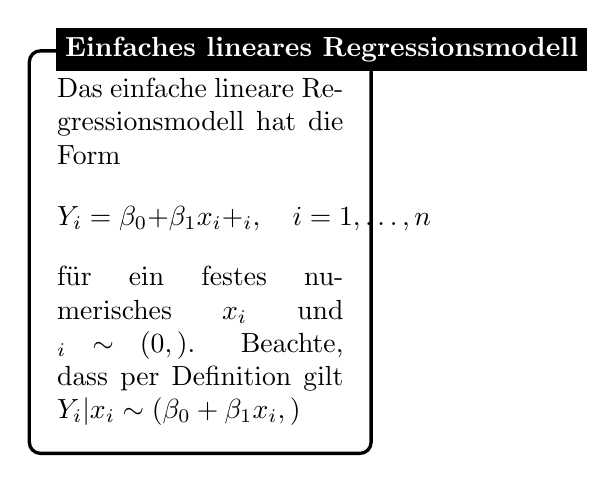
\begin{tikzpicture}
\node [mybox] (box){%
    \begin{minipage}{0.3\textwidth}
    Das \tc{einfache lineare Regressionsmodell} hat die Form 
    $$Y_i = \beta_0 + \beta_1 x_i + \eps_i,\quad i = 1, \dots, n$$
    für ein festes numerisches $x_i$ und $\eps_i \sim \Ncal(0,\ssd)$.
    Beachte, dass per Definition gilt $Y_i| x_i \sim \Ncal(\beta_0 + \beta_1 x_i, \ssd)$
    \end{minipage}
};
%------------ Einfaches lineares Regressionsmodell Header ---------------------
\node[fill = black, text=white, font=\bfseries, right=10pt] at (box.north west) 
{Einfaches lineares Regressionsmodell};
\end{tikzpicture}

%------------ KQ Schätzer ---------------
\begin{tikzpicture}
\node [mybox] (box){%
    \begin{minipage}{0.3\textwidth}
    Wir schätzen die Parameter $(\beta_0, \beta_1)$ durch 
    \begin{align}
        (\hbe0, \hbe1) = \argmin_{(\beta_0, \beta_1)} \sum_{i = 1}^n(Y_i - (\beta_0 + \beta_1 x_i))^2
    \end{align}
    und nennen $(\hbe0, \hbe1)$ den \tc{KQ-Schätzer von $(\beta_0, \beta_1)$} und 
    $\hat{\eps}_i := Y_i - (\hbe0 + \hbe1 x_i)$ die \tc{Residuen}.
    \end{minipage}
};
%------------ KQ Schätzer Header ---------------------
\node[fill = black, text=white, font=\bfseries, right=10pt] at (box.north west) 
{Kleinste Quadrate (KQ) Schätzer};
\end{tikzpicture}

%------------ Existenz und Berechnung vom KQ Schätzer ---------------
\begin{tikzpicture}
\node [mybox] (box){%
    \begin{minipage}{0.3\textwidth}
    Der KQ-Schätzer existiert und ist eindeutig, falls $\sum_{i = 1}^n (x_i - \bar{x})^2 \neq 0$. 
    Dieser lässt sich berechnen als 
    \begin{align*}
        \hbe1 = & \quad \frac{S_{xY}}{S_x^2} = 
        \frac{\frac1n\sum_{i = 1}^n (x_i - \bar{x})(Y_i - \bar{Y})}{\frac1n\sum_{i = 1}^n (x_i - \bar{x})^2}\\
        \hbe0 = & \quad \bar{Y} - \hbe1 \bar{x}.
    \end{align*}
    Durch differenzieren von der Gleichung (1) erhält man $(\hbe0, \hbe1)$ als Lösung der 
    \tc{Normalengleichungen}
    \begin{align*}
        \sumin \hat{\eps}_i = 0\\
        \sumin \hat{\eps}_i x_i = 0
    \end{align*}
    \end{minipage}
};
%------------ Existenz und Berechnung vom KQ Schätzer Header --------
\node[fill = purple, text=white, font=\bfseries, right=10pt] at (box.north west) 
{Existenz und Berechnung vom KQ Schätzer};
\end{tikzpicture}


%------------ Interpretation der Modellparameter ---------------
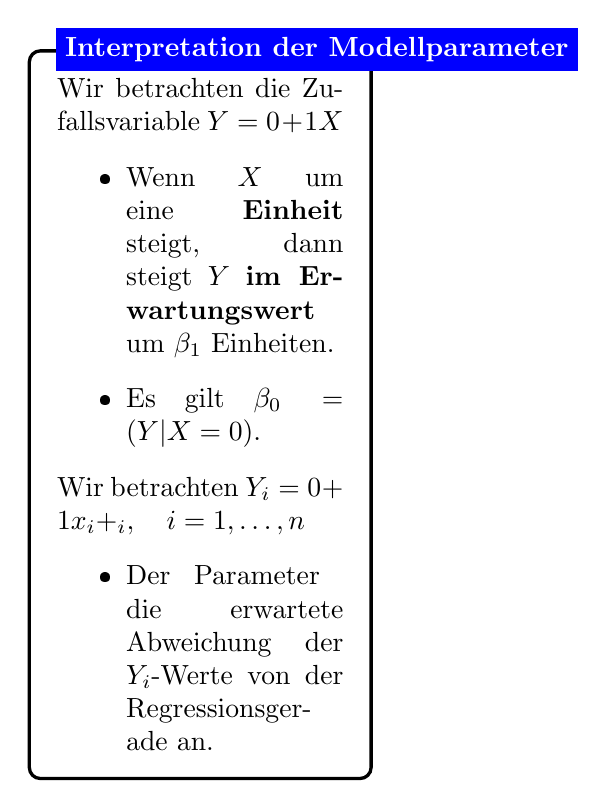
\begin{tikzpicture}
    \node [mybox] (box){%
        \begin{minipage}{0.3\textwidth}
        Wir betrachten die Zufallsvariable $Y = \gb0 + \gb1 X$
        \begin{itemize}
            \item Wenn $X$ um eine \textbf{Einheit} steigt, 
            dann steigt $Y$ \textbf{im Erwartungswert} um $\beta_1$ Einheiten.
            \item Es gilt $\beta_0 = \E(Y|X = 0)$.
        \end{itemize}
        Wir betrachten $Y_i = \gb0 + \gb1 x_i + \eps_i, \quad i = 1,\dots, n$
        \begin{itemize}
            \item Der Parameter $\sd$ die erwartete Abweichung der $Y_i$-Werte von der Regressionsgerade an.
        \end{itemize}
        \end{minipage}
    };
%------------ Interpretation der Modellparameter Header ---------------------
\node[fill = blue, text=white, font=\bfseries, right=10pt] at (box.north west) {Interpretation der Modellparameter};
\end{tikzpicture}
    

%------------ Eigenschaften des KQ-Schätzers ---------------
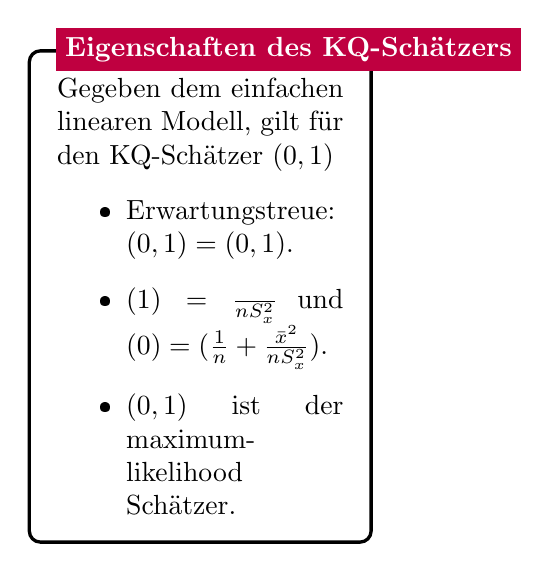
\begin{tikzpicture}
    \node [mybox] (box){%
        \begin{minipage}{0.3\textwidth}
        Gegeben dem einfachen linearen Modell, gilt für den KQ-Schätzer $(\hbe0,\hbe1)$
        \begin{itemize}
            \item Erwartungstreue: $\E(\hbe0,\hbe1) = (\gb0,\gb1)$.
            \item $\V(\hbe1) = \frac{\ssd}{nS_x^2}$ und $\V(\hbe0) = \ssd (\frac 1n + \frac{\bar{x}^2}{nS_x^2})$.
            \item $(\hbe0,\hbe1)$ ist der maximum-likelihood Schätzer.
        \end{itemize}
        \end{minipage}
    };
%------------ Eigenschaften des KQ-Schätzers Header ---------------------
\node[fill = purple, text=white, font=\bfseries, right=10pt] at (box.north west) {Eigenschaften des KQ-Schätzers};
\end{tikzpicture}


%------------ Schätzer für $\ssd$ ---------------
\begin{tikzpicture}
    \node [mybox] (box){%
        \begin{minipage}{0.3\textwidth}
        Gegeben dem einfachen linearen Modell mit\\$\eps_i \sim \Ncal(0,\ssd)$, gilt
        $$\hat{\sd}^2 := \frac{1}{n-2}\sumin \hat{\eps}_i^2$$ 
        ist ein erwartungstreuer Schätzer von $\ssd$ und 
        $$\frac{n-2}{\ssd}\hat{\sd}^2 \sim \chi_{n-2}^2.$$
        Der KQ-Schätzer $(\hbe0,\hbe1)$ und der Schätzer $\hat{\sd}^2$ sind stoch.unabhängig.
        \end{minipage}
    };
    %------------ chätzer für $\ssd$ Header ---------------------
    \node[fill = purple, text=white, font=\bfseries, right=10pt] at (box.north west) {Schätzer für $\ssd$};
    \end{tikzpicture}
    


%------------ Konfidenzintervalle für $\gb0$ und $\gb1$ ---------------
\begin{tikzpicture}
    \node [mybox] (box){%
        \begin{minipage}{0.3\textwidth}
        Gegeben dem einfachen linearen Modell mit\\$\eps_i \sim \Ncal(0,\ssd)$, gilt für $\hbe1$ und $\hbe0$
        $$\frac{\hbe1 - \gb1}{\hat{\sd}_{\hbe1}} \sim t_{n-2} \text{ mit } \hat{\sd}_{\hbe1} 
        := \sqrt{\frac{\hat{\sd}^2}{\sumin (x_i - \bar{x})^2}}$$
        $$\frac{\hbe0 - \gb0}{\hat{\sd}_{\hbe0}} \sim t_{n-2} \text{ mit } \hat{\sd}_{\hbe0} 
        := \sqrt{\hat{\sd}^2 \frac{\sumin x_i^2}{n\sumin (x_i - \bar{x})^2}}$$
        Damit können wir Konfidenzintervalle zum Niveau $1 - \alpha$ für $\gb1$ und $\gb0$ erzeugen:
        $$[\ \hbe1 - \hat{\sd}_{\hbe1}t_{1 - \alpha/2}(n-2); \hbe1 + \hat{\sd}_{\hbe1}t_{1 - \alpha/2}(n-2) ]\ $$
        $$ [\ \hbe0 - \hat{\sd}_{\hbe0}t_{1 - \alpha/2}(n-2); \hbe0 + \hat{\sd}_{\hbe0}t_{1 - \alpha/2}(n-2) ]\ $$
        \end{minipage}
    };
    %------------  Konfidenzintervalle für $\gb0$ und $\gb1$ Header ---------------------
    \node[fill = purple, text=white, font=\bfseries, right=10pt] at (box.north west) 
    {Konfidenzintervalle für $\gb0$ und $\gb1$};
    \end{tikzpicture}

%------------ Quadratsummenzerlegung ---------------
\begin{tikzpicture}
    \node [mybox] (box){%
        \begin{minipage}{0.3\textwidth}
        Gegeben sei ein einfaches linearen Modell mit\\$\eps_i \sim \Ncal(0,\ssd)$ und 
        $\hat{Y}_i := \hbe0 + \hbe1x_i$. Dann gilt
        $$ \underbrace{\sumin (Y_i - \bar{Y})^2}_{\text{SST}} = \underbrace{\sumin (Y_i - \hat{Y}_i)^2}_{\text{SSE}} 
        - \underbrace{\sumin(\hat{Y}_i - \bar{Y})^2}_{\text{SSM}} .$$
        \begin{align*}
            & \text{SST(otal):} & \text{Gesamtstreuung von Y}\\
            & \text{SSE(rror):} & \text{Streuung der Residuen}\\
            & \text{SSM(odel):} & \text{Streuung, die das Modell erklärt}\\
        \end{align*}
        \end{minipage}
    };
%------------ Quadratsummenzerlegung Header ---------------------
\node[fill = purple, text=white, font=\bfseries, right=10pt] at (box.north west) {Quadratsummenzerlegung};
\end{tikzpicture}
    
%------------ Bestimmtheitsmaß ---------------
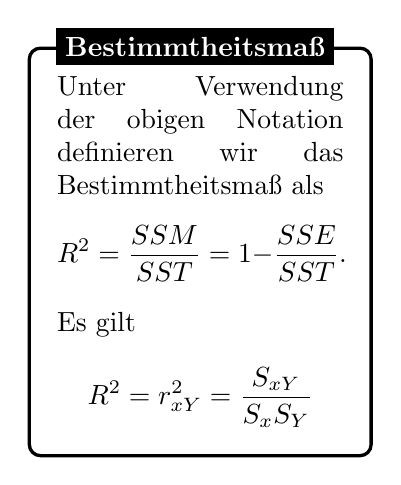
\begin{tikzpicture}
    \node [mybox] (box){%
        \begin{minipage}{0.3\textwidth}
        Unter Verwendung der obigen Notation definieren wir das \tc{Bestimmtheitsmaß} als
        $$R^2 = \frac{\text{SSM}}{\text{SST}} = 1 - \frac{\text{SSE}}{\text{SST}}.$$
        Es gilt $$R^2 = r_{xY}^2 = \frac{S_{xY}}{S_xS_Y}$$
        \end{minipage}
    };
    %------------ Bestimmtheitsmaß Header ---------------------
    \node[fill = black, text=white, font=\bfseries, right=10pt] at (box.north west) {Bestimmtheitsmaß};
    \end{tikzpicture}




%------------ Überschrift ---------------

\begin{tikzpicture}
\node [mybox] (box){%
    \begin{minipage}{0.3\textwidth}
    
    \end{minipage}
};
%------------ Überschrift Header ---------------------
\node[fill = black, text=white, font=\bfseries, right=10pt] at (box.north west) {Überschrift};
\end{tikzpicture}







\end{multicols*}